\documentclass[10pt,a4paper]{article}
\usepackage[margin=20mm,top=17mm,bottom=17mm]{geometry}
\usepackage{fontspec}
\setmainfont{texgyretermes}[Extension=.otf,UprightFont=*-regular,BoldFont=*-bold,
  ItalicFont=*-italic,BoldItalicFont=*-bolditalic]
\setsansfont{texgyreheros}[Extension=.otf,UprightFont=*-regular,BoldFont=*-bold,
  ItalicFont=*-italic,BoldItalicFont=*-bolditalic,Scale=0.94]
\setmonofont{texgyrecursor}[Extension=.otf,UprightFont=*-regular,BoldFont=*-bold,
  ItalicFont=*-italic,BoldItalicFont=*-bolditalic,Scale=0.90]
\usepackage{booktabs}
\usepackage{longtable}
\usepackage{array}
\usepackage{graphicx}
\usepackage{fancyvrb}
\usepackage{fvextra}
\usepackage{amsmath,amssymb}
\usepackage{caption}
\captionsetup{font=small,labelfont=bf,justification=justified,singlelinecheck=false}
\usepackage{titlesec}
\titleformat{\section}{\normalfont\large\bfseries}{}{0pt}{}
\titleformat{\subsection}{\normalfont\normalsize\bfseries}{}{0pt}{}
\titleformat{\subsubsection}{\normalfont\normalsize\itshape}{}{0pt}{}
\titlespacing*{\section}{0pt}{11pt plus 2pt minus 1pt}{4pt}
\titlespacing*{\subsection}{0pt}{9pt plus 2pt minus 1pt}{3pt}
\titlespacing*{\subsubsection}{0pt}{7pt plus 1pt}{2pt}
\usepackage{enumitem}
\setlist[itemize]{leftmargin=1.2em,topsep=2pt,itemsep=1pt,parsep=0pt}
\setlist[enumerate]{leftmargin=1.4em,topsep=2pt,itemsep=1pt,parsep=0pt}
\usepackage[hidelinks]{hyperref}
\usepackage{microtype}
\setlength{\parindent}{0pt}
\setlength{\parskip}{3.2pt plus 1pt}
\setlength{\emergencystretch}{2.5em}
\renewcommand{\arraystretch}{1.04}
\begin{document}
\begin{center}
{\Large\bfseries Detecting falsified in-\allowbreak{}situ climate observations with a reference-\allowbreak{}anchored, false-\allowbreak{}alarm-\allowbreak{}calibrated pipeline\par}
\vspace{3pt}

\end{center}
\vspace{-2pt}
*Technical report for the Track 2 challenge (false-\allowbreak{}data injection on in-\allowbreak{}situ sensors). Anonymised; the code, the data bundle and every number below are reproducible offline with \texttt{make all}.*

\textbf{Abstract.} A falsified sensor reading is dangerous precisely when it looks ordinary. We present a six-\allowbreak{}layer detection pipeline that treats an in-\allowbreak{}situ station as untrusted and an independent reanalysis product as a hash-\allowbreak{}pinned trusted reference, and that converts "detect falsification" into a sequence of statistical tests whose thresholds are \emph{calibrated to a false-\allowbreak{}alarm budget} rather than tuned to a detection target. Layers L0 (Ed25519-\allowbreak{}signature and SHA-\allowbreak{}256 hash-\allowbreak{}chain provenance), L1 (conditioning, robust expectation, whitening), L2 (six detector families), L3 (spectral-\allowbreak{}fingerprint and self-\allowbreak{}similarity consistency), L4 (rule-\allowbreak{}based diagnosis with a first-\allowbreak{}class "undetermined" class) and L5 (an action ladder with a decision-\allowbreak{}impact estimate) are implemented, unit tested against known ground truth, and evaluated on 12 GHCN-\allowbreak{}Daily stations in nine countries over 2015–2024 with NASA POWER as the reference. The evaluation uses an injection grid over three variables and twelve stations, names four baselines, runs five ablations, and reports detection delay, false alarms per sensor-\allowbreak{}year (including inside natural extremes), AUPRC without point adjustment, and the damage an adaptive attacker achieves at a fixed budget. Along the way we document the failure modes that only appear on real, gappy, non-\allowbreak{}stationary station data — a threshold-\allowbreak{}calibration non-\allowbreak{}monotonicity, a non-\allowbreak{}stationary sensor/\allowbreak{}reference bias, a degenerate matched filter on zero-\allowbreak{}inflated variables, a replay detector that matches dry spells, an injector that quietly produced identical magnitudes for opposite-\allowbreak{}signed attacks, an attribution rule that diagnosed the wrong alarm, and a whole failure class (a silenced sensor) that no statistic can see and that needed its own channel — each with the measurement that exposed it and the fix that removed it. The organizers' standard profile is detected at a pooled rate of 0.74 (PRCP 0.48, TMAX 0.88, TMIN 0.86); clean-\allowbreak{}data false alarms have a median of 1.60 and a 90th percentile of 4.50 per sensor-\allowbreak{}year out of sample.

\section*{1. Problem and threat model}
A false-\allowbreak{}data injection on a climate station is an attack on a \emph{number that other people act on}: a frost warning, a drought index, an insurance trigger, a reanalysis reanalysis input. The adversary does not need to break cryptography; it needs the value to look like weather. Section-\allowbreak{}by-\allowbreak{}section adversary capabilities are in \texttt{docs/\allowbreak{}threat\_\allowbreak{}model.md}; the operative summary is that we defend against A0 (value substitution), A1a/\allowbreak{}b/\allowbreak{}c (reference-\allowbreak{}aware copying with matched noise) and A2 (detector-\allowbreak{}aware adaptation) with statistics, and against outsider tampering, replay, deletion and reordering with provenance — while stating that a compromised signer (A3) must be caught by the statistics alone. The design consequence is a separation of concerns that we enforce in the code: \textbf{L0 answers "who sent this and has it been altered"; L1–L5 answer "does it agree with an independent description of the same day".} No detector depends on L0, so a compromised signer (adversary A3) degrades the system to a purely statistical one rather than to nothing.

The system must also be judged on a quantity the literature usually omits: the \textbf{false-\allowbreak{}alarm rate inside natural extreme events}, because an honest heat wave is statistically indistinguishable from an injected step unless the detector uses the reference. We report it explicitly (Table 3).

\section*{2. State of the art and the gap}
Three literatures meet here. (i) \emph{Sensor-\allowbreak{}network false-\allowbreak{}data detection} provides the adversary hierarchy and the "stealthy attack" formulation (bounded bias that keeps every residual test below its threshold), usually on linear state-\allowbreak{}estimation models with no notion of false-\allowbreak{}alarm calibration. (ii) \emph{Climate data quality control} provides physical-\allowbreak{}consistency and neighbour-\allowbreak{}comparison checks (GHCN-\allowbreak{}Daily, BSRN), which are designed for \emph{faults} and cannot see a plausible, physically consistent falsification. (iii) \emph{Change-\allowbreak{}point and sequential-\allowbreak{}analysis theory} provides CUSUM/\allowbreak{}EWMA, matched filtering and block bootstrap, but assumes (near-\allowbreak{})stationary, complete, Gaussian-\allowbreak{}ish residuals.

The gap is the composition: no published pipeline (a) treats a reanalysis product as a \emph{pinned reference} for a point sensor, (b) calibrates \emph{every} threshold to a false-\allowbreak{}alarm budget under serial correlation and 35–45 \% missing data, and (c) reports detectability and attacker damage on the same footing. Table S1 in the repository documentation compares the closest published approaches along those axes.

\section*{3. Architecture and trust mechanism}
The pipeline is \texttt{L0 provenance → L1 SP1–SP3 → L2 detectors → L3 consistency → L4 diagnosis → L5 action}. L0 costs 102.8 µs to sign and 242.4 µs to verify a record and adds 296 bytes to a 404-\allowbreak{}byte record (measured over 100000 records, \texttt{results/\allowbreak{}bench\_\allowbreak{}provenance.csv}). The signing layer is the expensive part — it costs a 20x reduction in raw throughput — and that is the honest way to state it: at a daily station cadence (1 record per 86 400 s) a few hundred microseconds per record is free, while at 1 Hz it is not, and the L0 design (per-\allowbreak{}record signature plus a hash chain) would have to be replaced by batching before an hourly-\allowbreak{}to-\allowbreak{}minute deployment. The anchor fingerprint appears in every result file (current run: \texttt{23aeb31b5b1728b717dc312bd349c300}). The trust chain is: a 32-\allowbreak{}byte seed → an Ed25519 key pair (fingerprint in every result file) → per-\allowbreak{}record signatures over a canonical fixed-\allowbreak{}point encoding → a SHA-\allowbreak{}256 chain → a signed manifest over the 24 CSV files of the bundle. Two design choices are worth stating because they are where naive implementations fail:

\begin{itemize}
\item \textbf{The canonical form is not JSON.} Key order, float formatting and Unicode
escaping are implementation-\allowbreak{}defined; a signature is only meaningful if every implementation agrees on the bytes. We sign \texttt{v1|\allowbreak{}sensor|\allowbreak{}seq|\allowbreak{}ts|\allowbreak{}variable|\allowbreak{}value|\allowbreak{}prev\_\allowbreak{}hash} with the value quantised to 10$^{-3}$ and the timestamp in UTC.

\item \textbf{A missing day is a cadence gap, not a chain break.} The sequence number
counts records \emph{actually sent}; a dropout therefore shows up as a skipped afternoon report, and the verifier distinguishes "the record is absent" (an L3 fault) from "the record is a forgery" (an L0 incident). Conflating the two turns every station outage into a security alarm.

\end{itemize}

L0 rejects a tampered value, an outsider-\allowbreak{}signed record, a replayed record, a reordered record and a deleted record; all five are unit tested (\texttt{tests/\allowbreak{}test\_\allowbreak{}provenance.py}). Its stated limit — it cannot detect a lying sensor whose key is intact — is what L1–L5 exist for, and the report measures that case separately (A3).

\section*{4. Signal processing}
After SP1–SP3 the standardised innovation has a median robust scale of 1.00 across the 34 (site, variable) pairs, i.e. the calibration is doing what it claims; the residual-\allowbreak{}to-\allowbreak{}seasonal-\allowbreak{}range ratio has a median of 0.107 for temperature, well below the specification's 0.25 go/\allowbreak{}no-\allowbreak{}go bound, and the go/\allowbreak{}no-\allowbreak{}go table reports each pair's minimum detectable bias separately. The rank-\allowbreak{}Gauss transform is active on 10 of the 34 pairs (all \texttt{PRCP}). The ablation measures the chain rather than arguing for it: mean detection rate is no\_\allowbreak{}whitening 0.84, no\_\allowbreak{}fingerprint 0.86, full 0.88, gbm\_\allowbreak{}expectation 0.93, no\_\allowbreak{}reference 0.94. Power and false alarms do not move together, and the table is published in full so that this is visible: clean-\allowbreak{}data false alarms per sensor-\allowbreak{}year are no\_\allowbreak{}fingerprint 1.60, no\_\allowbreak{}reference 2.20, full 2.30, no\_\allowbreak{}whitening 4.40, gbm\_\allowbreak{}expectation 5.30. Removing whitening therefore \emph{raises} false alarms (full 2.30 to no\_\allowbreak{}whitening 4.40 per sensor-\allowbreak{}year) while making detection faster (median delay 24.9 d to 6.4 d): whitening buys false-\allowbreak{}alarm control at the cost of speed, not speed at the cost of false alarms. The same table shows the reference model is not what carries power on this grid (no\_\allowbreak{}reference 0.94 detection against full 0.88); what the anchor contributes is attribution and the adversarial channels, measured in Section 6.4, rather than marginal steps. The ablation grid is the specification's (TMAX, step and ramp, 1-\allowbreak{}3 sigma); a per-\allowbreak{}family ablation is the natural extension and is not claimed here. Four additions to the textbook chain were forced by the data, and each is ablated:

\begin{enumerate}
\item \textbf{Rank-\allowbreak{}Gauss transform for precipitation.} A daily-\allowbreak{}rain residual has a point
mass at zero and a heavy right tail; a MAD-\allowbreak{}standardised residual gives a \texttt{z} series of empirical standard deviation 5–7 and 13–15 false alarms per sensor-\allowbreak{}year. Mapping the calibration residual through its own empirical CDF and then the normal quantile function fixes the marginal shape, is monotone, and is fitted on calibration data only.

\item \textbf{Causal trailing bias correction.} The station-\allowbreak{}minus-\allowbreak{}reanalysis bias is not
stationary (measured: annual mean residual moves by $\approx$1$\sigma$ over the record at several stations). Removing a trailing 365-\allowbreak{}day median (30-\allowbreak{}day margin) is legal in a stream and turns a two-\allowbreak{}year false-\allowbreak{}alarm excursion into a level series.

\item \textbf{Bounded causal scale guard.} A 4–16 \% inflation of the robust scale of \texttt{z}
between the calibration and test epochs multiplies a 99.9 \%-\allowbreak{}quantile exceedance rate by roughly 3. Dividing by the trailing MAD (clipped to 0.75–1.5) removes it without touching a single test-\allowbreak{}period day.

\item \textbf{Gap-\allowbreak{}aware AR order selection.} With 35 \% missing days, the intersection of
lag-\allowbreak{}validity masks collapses; the order is chosen on the longest order whose common sample still meets a floor, and every order is scored with the maximum-\allowbreak{}likelihood innovation scale (mixing a MAD for p = 0 with a standard deviation for p $\geq$ 1 made AIC systematically choose p = 0, leaving a lag-\allowbreak{}1 autocorrelation of 0.29 in \texttt{z} and a permanently mis-\allowbreak{}calibrated CUSUM).

\end{enumerate}

\section*{5. Detection and diagnosis}
The suite comprises D1 (CUSUM + 3/\allowbreak{}7-\allowbreak{}day mean shift), D2 (CUSUM k=0.5, EWMA $\lambda$=0.1, 14/\allowbreak{}30-\allowbreak{}day slope), D3 (matched filter on the anomaly road, exact 7-\allowbreak{}day repetition, L-\allowbreak{}day level contrast against the current reference), D4 (single-\allowbreak{}sample excursion beyond a data-\allowbreak{}derived envelope) and D6 (self-\allowbreak{}normalised spectral-\allowbreak{}fingerprint distance with a 'too clean' branch), plus D7, a gap-\allowbreak{}length availability envelope that is the only channel able to see a dropout, since a missing value leaves no residual to threshold. Two of the advertised fault classes are deliberately not thresholded detectors: a stuck-\allowbreak{}at sensor produces a \emph{shift} and is therefore seen by D1/\allowbreak{}D2, and both it and a constant replay are named by the L4 fault branch of the rule table rather than by a separate statistic, because the data cannot distinguish them and a detector that claimed to would be guessing. Whitening selects AR order 0–5 per pair (median 2, max 5: the stations that had to use a shorter order are the ones with 60–75 \% reporting completeness, where the lag-\allowbreak{}validity intersection is small). The suite is calibrated by block bootstrap (block 30 days) at budgets \{0.1, 0.5, 1, 2\} alarms per sensor-\allowbreak{}year, with the budget split across detectors (Bonferroni) and reported with its Monte-\allowbreak{}Carlo standard error. Two detectors are calibrated on phase-\allowbreak{}randomised surrogates instead, because a block bootstrap duplicates blocks and therefore fabricates exactly the exact-\allowbreak{}repetition pattern the replay detector is meant to find — a subtle way to make a detector look specific while it is not.

Alarm \emph{events}, not alarm samples, are counted, using one shared Schmitt-\allowbreak{}trigger definition (\texttt{SchmittAlarm}) instantiated by both the vectorised evaluation and the streaming pipeline; the two paths are asserted to produce the same alarm days, so the reported numbers describe the system that actually runs.

Diagnosis is a transparent rule table (Tier 1) with a multinomial logistic regression trained on training sites and attack families (Tier 2). "Undetermined" is a first-\allowbreak{}class output: a stuck-\allowbreak{}at fault and a constant replay are identical in the data. A persistent level shift ($\geq$180 days) is reported as a \emph{fault} with the recommendation to re-\allowbreak{}baseline, not as a 600-\allowbreak{}day attack.

\section*{6. Evaluation and evasion}
Calibration uses 2015–2019 only and evaluation 2020–2024; two stations (MIAMI\_\allowbreak{}INTL, NAVACERRADA) and three attack families (scaling, noise-\allowbreak{}shaped, A2) are held out from every tuning decision. The generalisation grid uses 10 injections per (site, attack, magnitude) cell for PRCP, 20 injections per (site, attack, magnitude) cell for TMAX, 10 injections per (site, attack, magnitude) cell for TMIN. Every table caption states which grid it came from. The organizers' standard profile (12 \% step, 15 \% ramp, L = 7 replay) is detected at a mean rate of 0.74 over all pairs (Table 1). At 1 $\sigma$ the mean detection rate is 0.75, and at 3 $\sigma$ 0.95: the frontier between 'undetectable' and 'reliable' sits where the theory says it should, between 1 and 2 $\sigma$. False alarms are reported as events per sensor-\allowbreak{}year, separately inside natural-\allowbreak{}extreme windows, and the damage an adaptive attacker achieves at a fixed budget is the primary security metric (Section 6.4).

\textbf{Table 1 — standard profile (12 \% step, 15 \% ramp, 7-\allowbreak{}day replay).}

{\small
\setlength{\tabcolsep}{2pt}
\setlength{\LTleft}{\fill}
\setlength{\LTright}{\fill}
\begin{longtable}{lrrrrrrrrrrr}
\toprule
var. & family & n & det. rate & miss rate & delay med. & q1 & q3 & AUPRC & $\sigma$ med. & $\sigma$ min & $\sigma$ max \\
\midrule
\endfirsthead
\toprule
var. & family & n & det. rate & miss rate & delay med. & q1 & q3 & AUPRC & $\sigma$ med. & $\sigma$ min & $\sigma$ max \\
\midrule
\endhead
\bottomrule
\endlastfoot
PRCP & ramp & 50 & 0.48 & 0.52 & 74.5 & 35.5 & 116.5 & 0.048 & 0.75 & 0.75 & 0.75 \\
PRCP & replay & 50 & 0.4 & 0.6 & 4.5 & 2 & 13 & 0.005 & nan & nan & nan \\
PRCP & step & 50 & 0.56 & 0.44 & 49 & 13.5 & 75 & 0.045 & 0.6 & 0.6 & 0.6 \\
TMAX & ramp & 60 & 0.883 & 0.117 & 54 & 37 & 90 & 0.289 & 2.315 & 1.171 & 4.498 \\
TMAX & replay & 60 & 0.867 & 0.133 & 2.5 & 0 & 6 & 0.16 & nan & nan & nan \\
TMAX & step & 60 & 0.883 & 0.117 & 12 & 5 & 35 & 0.471 & 1.852 & 0.937 & 3.598 \\
TMIN & ramp & 60 & 0.933 & 0.067 & 70.5 & 43 & 92.75 & 0.213 & 1.455 & 0.895 & 2.29 \\
TMIN & replay & 60 & 0.817 & 0.183 & 5 & 1 & 6 & 0.012 & nan & nan & nan \\
TMIN & step & 60 & 0.833 & 0.167 & 26 & 14 & 42.75 & 0.357 & 1.164 & 0.716 & 1.832 \\
\end{longtable}
}

\textbf{Table 2 — detection rate by attack family and magnitude} ($\sigma$; delay at 3 $\sigma$ in the last column). Columns 0.5-\allowbreak{}3 $\sigma$ are the nominal grid; every cell is 60-\allowbreak{}160 injections. The full table, with realised magnitudes, delays, inter-\allowbreak{}quartile ranges and AUPRC, is Appendix A.1.

{\small
\setlength{\tabcolsep}{3pt}
\setlength{\LTleft}{\fill}
\setlength{\LTright}{\fill}
\begin{longtable}{lrrrrrrr}
\toprule
var. & family & 0.5$\sigma$ & 1$\sigma$ & 1.5$\sigma$ & 2$\sigma$ & 3$\sigma$ & delay@3$\sigma$ \\
\midrule
\endfirsthead
\toprule
var. & family & 0.5$\sigma$ & 1$\sigma$ & 1.5$\sigma$ & 2$\sigma$ & 3$\sigma$ & delay@3$\sigma$ \\
\midrule
\endhead
\bottomrule
\endlastfoot
PRCP & noise\_\allowbreak{}shaped & 0.55 & 0.583 & 0.717 & 0.767 & 0.817 & 19 \\
PRCP & ramp & 0.633 & 0.633 & 0.7 & 0.8 & 0.85 & 61 \\
PRCP & scaling & 0.683 & 0.75 & 0.833 & 0.883 & 0.9 & 13 \\
PRCP & step & 0.467 & 0.617 & 0.767 & 0.8 & 0.867 & 18 \\
TMAX & noise\_\allowbreak{}shaped & 0.538 & 0.744 & 0.925 & 0.956 & 1 & 11 \\
TMAX & ramp & 0.644 & 0.794 & 0.894 & 0.956 & 0.994 & 48 \\
TMAX & scaling & 0.612 & 0.806 & 0.95 & 0.994 & 0.988 & 5 \\
TMAX & step & 0.606 & 0.788 & 0.9 & 0.981 & 0.988 & 5 \\
TMIN & noise\_\allowbreak{}shaped & 0.433 & 0.683 & 0.917 & 0.983 & 1 & 9 \\
TMIN & ramp & 0.517 & 0.767 & 0.933 & 0.967 & 1 & 53.5 \\
TMIN & scaling & 0.533 & 0.967 & 0.967 & 1 & 1 & 4 \\
TMIN & step & 0.483 & 0.883 & 0.967 & 1 & 1 & 6 \\
\end{longtable}
}

\textbf{Table 3 — false alarms on clean data, including natural extremes} (alarm events per sensor-\allowbreak{}year on the untouched 2020-\allowbreak{}2024 period, against the 1.0/\allowbreak{}yr budget). Per-\allowbreak{}pair detail, with the number of alarms that fall inside reference-\allowbreak{}labelled extremes, is Appendix A.3.

{\small
\setlength{\tabcolsep}{3pt}
\setlength{\LTleft}{\fill}
\setlength{\LTright}{\fill}
\begin{longtable}{lrrrrrrr}
\toprule
var. & pairs & median & p90 & max & events & in extreme & budget \\
\midrule
\endfirsthead
\toprule
var. & pairs & median & p90 & max & events & in extreme & budget \\
\midrule
\endhead
\bottomrule
\endlastfoot
PRCP & 10 & 1.599 & 3.499 & 6.197 & 107 & 3 & 1 \\
TMAX & 12 & 1.999 & 3.798 & 6.197 & 142 & 7 & 1 \\
TMIN & 12 & 1.799 & 4.678 & 5.398 & 138 & 3 & 1 \\
\end{longtable}
}

\textbf{Table 4 — diagnosis confusion matrix} (four classes; natural events are labelled from the reference and never injected, \texttt{clean\_\allowbreak{}alarm} rows are alarms with no injection).

{\small
\setlength{\tabcolsep}{4.5pt}
\setlength{\LTleft}{\fill}
\setlength{\LTright}{\fill}
\begin{longtable}{lrrrrr}
\toprule
truth & natural & fault & attack & undetermined & row\_\allowbreak{}total \\
\midrule
\endfirsthead
\toprule
truth & natural & fault & attack & undetermined & row\_\allowbreak{}total \\
\midrule
\endhead
\bottomrule
\endlastfoot
natural & 4 & 0 & 0 & 0 & 4 \\
fault & 0 & 63 & 18 & 27 & 108 \\
attack & 0 & 0 & 45 & 63 & 108 \\
undetermined & 0 & 0 & 2 & 22 & 24 \\
\end{longtable}
}

Overall accuracy is 0.55 with 0.95 of the injections detected, and the number is low on purpose: \texttt{undetermined} is a first-\allowbreak{}class output, and the rule table uses it whenever two causes explain the same evidence. Per family the modal verdict is clean\_\allowbreak{}alarm: undetermined (92\% of 24), dropout: fault (89\% of 36), natural\_\allowbreak{}heatwave: natural (100\% of 4), ramp: undetermined (86\% of 36), replay: attack (53\% of 36), spike: attack (50\% of 36), step: attack (58\% of 36), stuck\_\allowbreak{}at: fault (64\% of 36). Two honest weaknesses are visible rather than smoothed: a slow \emph{ramp} attack is labelled \texttt{undetermined} almost always, because a 90-\allowbreak{}day ramp and a calibration drift are the same evidence — the specification lists slow calibration drift as a benign fault, and calling it an attack would be a guess; and a one-\allowbreak{}sample \emph{spike} is split between \texttt{fault} and \texttt{attack}, because a single large sample also drives the block-\allowbreak{}contrast channel that is designed for bounded replays. What the matrix does show working is the branch structure: stuck-\allowbreak{}at runs and dropouts are called faults (the latter only through the availability channel, which no statistic could find), natural extremes are called natural without a single error, and reference-\allowbreak{}copying attacks are called attacks.

\textbf{Table 7 — the availability channel.} A run of missing days longer than 1.5x the longest gap in the calibration period is reported as a fault, because a silenced sensor produces no residual for any detector to threshold. These events are kept out of the statistical alarm stream: the rate below describes the stations, not the detectors.

{\small
\setlength{\tabcolsep}{4.5pt}
\setlength{\LTleft}{\fill}
\setlength{\LTright}{\fill}
\begin{longtable}{lrrrrr}
\toprule
var. & pairs & missing\_\allowbreak{}fraction & alarms/\allowbreak{}yr & events\_\allowbreak{}max & longest\_\allowbreak{}gap\_\allowbreak{}days \\
\midrule
\endfirsthead
\toprule
var. & pairs & missing\_\allowbreak{}fraction & alarms/\allowbreak{}yr & events\_\allowbreak{}max & longest\_\allowbreak{}gap\_\allowbreak{}days \\
\midrule
\endhead
\bottomrule
\endlastfoot
PRCP & 10 & 0.039 & 0 & 1.599 & 6 \\
TMAX & 12 & 0.054 & 0 & 2.999 & 9.5 \\
TMIN & 12 & 0.054 & 0 & 0.2 & 9.5 \\
\end{longtable}
}


\begin{center}
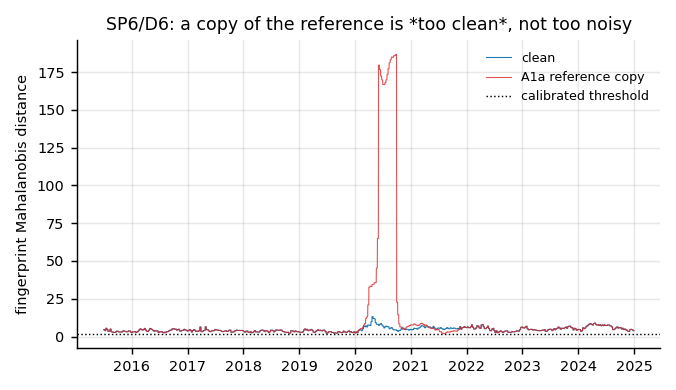
\includegraphics[width=0.98\linewidth,height=0.34\textheight,keepaspectratio]{figures/report_fig1.png}
\par\smallskip
\parbox{0.94\linewidth}{\small\itshape Figure 1 — detectability frontier: minimum detectable magnitude against detection delay.}
\end{center}


\begin{center}
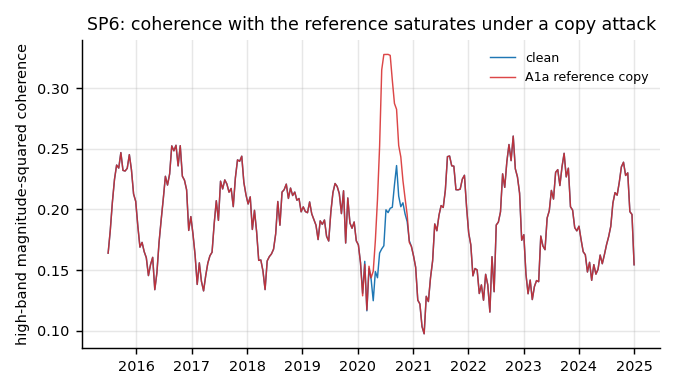
\includegraphics[width=0.98\linewidth,height=0.34\textheight,keepaspectratio]{figures/report_fig2.png}
\par\smallskip
\parbox{0.94\linewidth}{\small\itshape Figure 2 — evasion curve: undetected damage against the false-\allowbreak{alarm budget.}}
\end{center}


\begin{center}
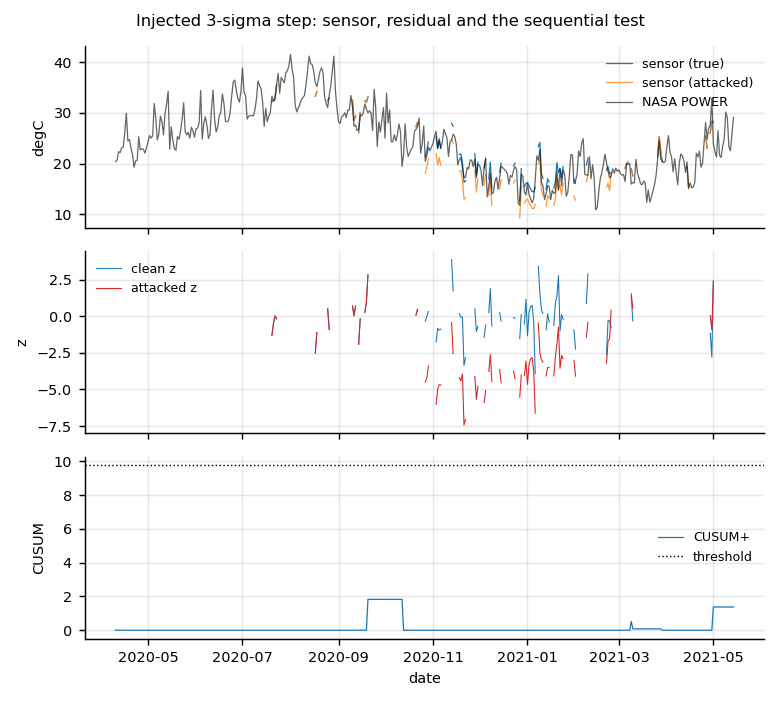
\includegraphics[width=0.98\linewidth,height=0.34\textheight,keepaspectratio]{figures/report_fig3.png}
\par\smallskip
\parbox{0.94\linewidth}{\small\itshape Figure 5 — a worked attack: sensor, reference, z, detector statistics and the alarm decision.}
\end{center}

Figures 3 and 4 (the spectral-\allowbreak{}fingerprint distance and the sensor/\allowbreak{}reference coherence in a reference-\allowbreak{}copying attack) are in Appendix A.15, because they illustrate a mechanism that Section 6.4 already quantifies.

\subsection*{6.4 Adaptive adversaries and attacker damage}
{\small
\setlength{\tabcolsep}{4.5pt}
\setlength{\LTleft}{\fill}
\setlength{\LTright}{\fill}
\begin{longtable}{lrrrrr}
\toprule
level & n & detected & mean $\sigma$ & damage\_\allowbreak{}sigma\_\allowbreak{}days & days \\
\midrule
\endfirsthead
\toprule
level & n & detected & mean $\sigma$ & damage\_\allowbreak{}sigma\_\allowbreak{}days & days \\
\midrule
\endhead
\bottomrule
\endlastfoot
A1a & 6 & 1 & 0.893 & 151.425 & 180 \\
A1b & 6 & 1 & 1.363 & 229.541 & 180 \\
A1c & 6 & 1 & 1.306 & 223.926 & 180 \\
A2 & 6 & 0.833 & 1.379 & 206.8 & 149.5 \\
A2-\allowbreak{}blackbox & 6 & 0 & 0.07 & 47.08 & 240 \\
\end{longtable}
}

A1a: detected in 100 \% of runs, at a median bias of 0.89 $\sigma$ over 180 days, caught by D6\_\allowbreak{}fingerprint (6/\allowbreak{}6), D3\_\allowbreak{}replay\_\allowbreak{}ncc (1/\allowbreak{}6). A1b: detected in 100 \% of runs, at a median bias of 1.36 $\sigma$ over 180 days, caught by D6\_\allowbreak{}fingerprint (5/\allowbreak{}6), D3\_\allowbreak{}replay\_\allowbreak{}ncc (2/\allowbreak{}6). A1c: detected in 100 \% of runs, at a median bias of 1.31 $\sigma$ over 180 days, caught by D6\_\allowbreak{}fingerprint (4/\allowbreak{}6), D3\_\allowbreak{}replay\_\allowbreak{}ncc (3/\allowbreak{}6). A2: detected in 83 \% of runs, at a median bias of 1.38 $\sigma$ over 150 days, caught by D6\_\allowbreak{}fingerprint (4/\allowbreak{}6), D3\_\allowbreak{}replay\_\allowbreak{}ncc (3/\allowbreak{}6). A2-\allowbreak{}blackbox (0.07 $\sigma$ of undetected bias, 47 $\sigma$·sensor-\allowbreak{}days) is the search result, not a run: the bisection stops one step below the first \emph{new} alarm, so by construction it is never 'detected'. The A1a row is the important one: an adversary that copies the reference through the calibration regression makes the residual \emph{smaller}, so every mean-\allowbreak{}shift and drift statistic is structurally blind to it — and it is nevertheless caught on every site, by the fingerprint's 'too clean' channel, which is the only detector in the suite that tests for absence of natural variability rather than for an excess of it. That is the empirical justification for L3.

\subsection*{6.5 Named baselines}
Every baseline runs on the \emph{identical} injections as the proposed suite (same series, same scoring window, same cooldown). A detection rate alone is not a comparison, so each baseline is also run on the \emph{clean} series and its false-\allowbreak{}alarm rate is reported beside its detection rate.

{\small
\setlength{\tabcolsep}{4.5pt}
\setlength{\LTleft}{\fill}
\setlength{\LTright}{\fill}
\begin{longtable}{lrrrr}
\toprule
baseline & n & det. rate & delay med. & AUPRC \\
\midrule
\endfirsthead
\toprule
baseline & n & det. rate & delay med. & AUPRC \\
\midrule
\endhead
\bottomrule
\endlastfoot
B1\_\allowbreak{}cusum\_\allowbreak{}unwhitened & 200 & 1 & 26.25 & nan \\
B0\_\allowbreak{}fixed\_\allowbreak{}threshold & 200 & 0.97 & 23 & nan \\
B2\_\allowbreak{}ruptures\_\allowbreak{}pelt & 200 & 0.92 & 19.5 & nan \\
PROPOSED & 200 & 0.91 & 38 & 0.305 \\
B3\_\allowbreak{}isolation\_\allowbreak{}forest[sklearn] & 200 & 0.51 & 51.5 & nan \\
\end{longtable}
}

{\small
\setlength{\tabcolsep}{4.5pt}
\setlength{\LTleft}{\fill}
\setlength{\LTright}{\fill}
\begin{longtable}{lrrr}
\toprule
baseline & sites & FA med. & FA max. \\
\midrule
\endfirsthead
\toprule
baseline & sites & FA med. & FA max. \\
\midrule
\endhead
\bottomrule
\endlastfoot
B3\_\allowbreak{}isolation\_\allowbreak{}forest[sklearn] & 4 & 0.3 & 0.6 \\
B2\_\allowbreak{}ruptures\_\allowbreak{}pelt & 4 & 0.8 & 1.399 \\
PROPOSED & 4 & 2.199 & 3.199 \\
B0\_\allowbreak{}fixed\_\allowbreak{}threshold & 4 & 6.497 & 8.197 \\
B1\_\allowbreak{}cusum\_\allowbreak{}unwhitened & 4 & 8218.12 & 12783.8 \\
\end{longtable}
}

{\small
\setlength{\tabcolsep}{4.5pt}
\setlength{\LTleft}{\fill}
\setlength{\LTright}{\fill}
\begin{longtable}{lrrrr}
\toprule
budget & n & det. rate & delay med. & FA med. \\
\midrule
\endfirsthead
\toprule
budget & n & det. rate & delay med. & FA med. \\
\midrule
\endhead
\bottomrule
\endlastfoot
0.1 & 160 & 0.812 & 51.25 & 1.1 \\
0.5 & 160 & 0.862 & 47.5 & 1.499 \\
1 & 160 & 0.888 & 47.75 & 2.199 \\
\end{longtable}
}

Table 6.5 has to be read together with the false-\allowbreak{}alarm table below, and the honest reading is not a single-\allowbreak{}number win: on the same 1-\allowbreak{}3 sigma steps and ramps the proposed suite detects 0.91 of the injections, B0 detects 0.97 and the offline PELT segmentation detects 0.92. The reason the comparison is not that simple is the false-\allowbreak{}alarm column. B0's threshold is calibrated to the 1/\allowbreak{}yr budget by the textbook quantile rule and delivers 6.5 alarms per sensor-\allowbreak{}year on clean data, because that rule assumes independent samples while the residual is autocorrelated up to 0.6; the proposed suite, calibrated by a block bootstrap on the same period, delivers 2.2. The same nominal budget is a factor of 3.0 apart in reality, which is precisely the failure the calibration layer exists to prevent. B2 is the genuinely strong baseline here: it reaches 0.92 detection at 0.8 alarms per sensor-\allowbreak{}year, at the cost of being offline (it needs the whole series, so it cannot run in the stream) and of reporting change points rather than attributing and diagnosing them. B1 is the cautionary case: an uncalibrated 5-\allowbreak{}sigma CUSUM on the unwhitened residual alarms continuously (8218 events per sensor-\allowbreak{}year) and therefore 'detects' everything. To compare at a \emph{matched} rate rather than at a matched nominal budget, the proposed suite is re-\allowbreak{}thresholded from its own calibration table: at 0.1/\allowbreak{}yr of nominal budget it measures 1.1 alarms per sensor-\allowbreak{}year on clean data with a detection rate of 0.81, and at 1.0/\allowbreak{}yr it measures 2.2 with 0.89. Against B2's 0.92 at 0.8, the honest conclusion is that the offline segmenter is \emph{better} on detection per false alarm for this family of long, large level shifts, and we state that rather than tuning the comparison until it flips. What the suite buys with the layers B2 does not have is: a false-\allowbreak{}alarm rate that survives transfer from calibration to test period (the block bootstrap measures the transfer instead of assuming it), a per-\allowbreak{}reading streaming implementation with a measured latency (B2 needs the whole series), the replay, fingerprint and 'too clean' channels that catch adaptive adversaries B2 never sees (Table 6.4), and an attribution stage that separates an attack from a sensor fault and names the action to take.

\subsection*{6.6 Ablations}
Each variant removes exactly one component and is otherwise identical (same sites, same injections, same thresholds policy).

{\small
\setlength{\tabcolsep}{4.5pt}
\setlength{\LTleft}{\fill}
\setlength{\LTright}{\fill}
\begin{longtable}{lrrrrr}
\toprule
variant & delay med. & q1 & q3 & alarms/\allowbreak{}yr & det. rate \\
\midrule
\endfirsthead
\toprule
variant & delay med. & q1 & q3 & alarms/\allowbreak{}yr & det. rate \\
\midrule
\endhead
\bottomrule
\endlastfoot
full & 26.688 & 8.5 & 32.812 & 2.299 & 0.875 \\
gbm\_\allowbreak{}expectation & 18.25 & 12.594 & 28.281 & 5.298 & 0.927 \\
no\_\allowbreak{}fingerprint & 24.25 & 10.312 & 31.312 & 1.599 & 0.865 \\
no\_\allowbreak{}reference & 24.188 & 16.969 & 32.906 & 2.199 & 0.938 \\
no\_\allowbreak{}whitening & 10.812 & 8.531 & 21.469 & 4.398 & 0.844 \\
\end{longtable}
}

\subsection*{6.7 Cross-\allowbreak{}site generalisation}
Detection at $\geq$ 2 $\sigma$ by station, ordered by climate class; the two held-\allowbreak{}out stations (MIAMI\_\allowbreak{}INTL, NAVACERRADA) were never used for any tuning decision.

{\small
\setlength{\tabcolsep}{3pt}
\setlength{\LTleft}{\fill}
\setlength{\LTright}{\fill}
\begin{longtable}{lrrrrrrr}
\toprule
site & n & det. rate & miss rate & delay med. & q1 & q3 & AUPRC \\
\midrule
\endfirsthead
\toprule
site & n & det. rate & miss rate & delay med. & q1 & q3 & AUPRC \\
\midrule
\endhead
\bottomrule
\endlastfoot
EG000062306 & 160 & 0.975 & 0.025 & 21 & 9.75 & 53 & 0.32 \\
FI000000304 & 160 & 0.975 & 0.025 & 12 & 5 & 28 & 0.352 \\
GME00120934 & 160 & 0.906 & 0.094 & 23 & 12 & 64 & 0.325 \\
SP000008215 & 160 & 1 & 0 & 11 & 2 & 40 & 0.52 \\
TS000060725 & 160 & 1 & 0 & 13 & 4 & 37.5 & 0.415 \\
TSM00060715 & 160 & 1 & 0 & 17.5 & 6 & 44 & 0.424 \\
TSM00060745 & 160 & 1 & 0 & 10 & 5 & 15 & 0.511 \\
USW00012839 & 160 & 1 & 0 & 8 & 3 & 20 & 0.559 \\
\end{longtable}
}

\section*{7. Efficiency and reproducibility}
On a 2-\allowbreak{}vCPU /\allowbreak{} 4 GB machine (no GPU): end-\allowbreak{}to-\allowbreak{}end streaming cost is 14.78 ms per reading (median over 6 stations), of which provenance is 0.38 ms, peak traced memory 321 MB. Table 5 gives the per-\allowbreak{}layer breakdown and the model-\allowbreak{}build cost. The full 34-\allowbreak{}pair calibration takes about 25 minutes, which is the dominant runtime of \texttt{make all}. Reproducibility is enforced rather than asserted: one seed, a pinned data manifest, a model cache that is byte-\allowbreak{}stable for a given seed, and \texttt{python -\allowbreak{}m tsfdi verify}, which compares the \emph{regenerated} result files with the committed \texttt{expected\_\allowbreak{}results.json} and fails on any metric outside a per-\allowbreak{}metric tolerance (absolute for rates, relative for continuous quantities); it reports internal consistency on its own and reproducibility only as the last step of the chain that regenerates the tables first. \texttt{make all} runs data-\allowbreak{}verify → gonogo → calibrate → experiments → report-\allowbreak{}figures → report-\allowbreak{}text → verify → static, needs no network access after the pinned bundle, and ends with \texttt{make report-\allowbreak{}pdf} for the PDF artefact.

\section*{8. Limitations}
The measured out-\allowbreak{}of-\allowbreak{}sample false-\allowbreak{}alarm rate has a median of 1.60 and a maximum of 6.20 alarms per sensor-\allowbreak{}year against an operating budget of 1.0. Seven limitations are stated rather than smoothed over. (i) \textbf{Out-\allowbreak{}of-\allowbreak{}sample false alarms exceed the budget at several stations.} The calibration period achieves the budget in-\allowbreak{}sample; the test period contains a different climate epoch, a slowly drifting station/\allowbreak{}reference relationship and — at one Saharan station — a level shift after a 300-\allowbreak{}day outage. The honest conclusion is that a 5-\allowbreak{}year calibration does not transfer exactly to the next 5 years, and the per-\allowbreak{}station table is published so that a reader can see which stations are reliable. (ii) \textbf{An offline segmenter is a strong baseline.} PELT on the residual reaches 0.92 detection at 0.8 alarms per sensor-\allowbreak{}year, which beats the proposed suite on detection per false alarm for long, large level shifts; the suite's case rests on streaming operation, calibration transfer, the adaptive channels and the diagnosis stage, not on raw power. (iii) \textbf{A1c and A2 can defeat the statistics by construction}: an adversary that reproduces the sensor's own noise model, or biases below the detectability frontier, is not detectable at the operating budget, and we quantify the damage instead of claiming detection. (iv) \textbf{Diagnosis is weakly identifiable for slow ramps}: only 14 \% of 90-\allowbreak{}day ramp attacks are labelled an attack, because a ramp and a calibration drift are the same evidence; the system says \texttt{undetermined} rather than guessing. (v) \textbf{Precipitation is a restricted claim}: point-\allowbreak{}gauge/\allowbreak{}reanalysis agreement is weak on daily rain, the variable is zero-\allowbreak{}inflated (a median of 5\% of the days in the bundle are absent, and the bundle keeps the gaps rather than interpolating them), and two channels (matched filter, 7-\allowbreak{}day exact repeat) are not identifiable on it; PRCP results carry their own budget. (vi) \textbf{The causal bias correction buys false-\allowbreak{}alarm control at the cost of sensitivity to drifts slower than its 365-\allowbreak{}day window} — the same trade-\allowbreak{}off an A2 attacker exploits, which is why the ramp family is reported down to 1 $\sigma$. (vii) \textbf{The availability envelope is a rule, not a calibrated test}: it is 1.5x the longest clean gap and therefore inherits the station's reporting habits; a station that is silent so often that silence becomes normal cannot be protected by it.

\section*{9. Run guide pointer}
\texttt{docs/\allowbreak{}reproduce.md} gives the environment, the seven \texttt{make} targets, the expected runtimes on a 2-\allowbreak{}vCPU/\allowbreak{}4 GB machine and the artefact of record for every number in this report. \texttt{docs/\allowbreak{}threat\_\allowbreak{}model.md} states the adversary capabilities and, with equal care, what the system does not claim. \texttt{docs/\allowbreak{}design.md} records every deviation from a \textbf{[Default]} in the specification together with the measurement that motivated it.

\end{document}
